\section{Auswertung}
\label{sec:Auswertung}

\subsection{Gegengekoppelter Verstärker}

Die Werte der vier verschiedenen Widerstandskombinationen sind in den Tabellen \ref{tab:gegen_kombi_1}, \ref{tab:gegen_kombi_2}, \ref{tab:gegen_kombi_3} und \ref{tab:gegen_kombi_4} eingetragen.
Die Fehler werden wie folgt angenommen: $\sigma_\nu = \num{0.1} \nu, \sigma_U = \SI{10}{\milli\volt}$. Graphisch dargestellt sind die Messwerte sowie ein Fit an die Messwerte, die händisch der Flanke zugeordnet werden, in Abbildung \ref{fig:gegen} zu sehen.
\begin{figure}
  \centering
  \includegraphics[width=1.2\textwidth]{build/gegen.pdf}
  \caption{Messwerte und Flankenfit aller vier Widerstandskombinationen mit $V'_\text{Theorie} = R_N / R_1$.}
  \label{fig:gegen}
\end{figure}
Dieser Fit folgt der Gleichung:
\begin{align}
  \ln(V') = m \ln(\nu/\si{\kilo\hertz}) + b.
\end{align}
Dabei ergeben sich die Werte aus Tabelle \ref{tab:gegen_ergebnisse}. Dort ist auch die Grenzfrequenz eingetragen, die aus dem Schnittpunkt der gefitteten Graden mit der Linie auf Höhe von $V'_\text{Theorie}/\sqrt{2}$ beziehungsweise $V'_\text{Theorie}\cdot\sqrt{2}$ gewonnen wird. Außerdem ist in Tabelle \ref{tab:gegen_ergebnisse} der Mittelwert der Messwerte der Plateaus angegeben, sowie die prozentuale Abweichung von $V'_\text{Theorie}$.

\begin{table}[h]
  \centering
  \begin{tabular}{S[table-format=1.0]
    S[table-format=2.3] @{${}\pm{}$} S[table-format=1.3]
    S[table-format=2.2] @{${}\pm{}$} S[table-format=1.2]
    S[table-format=3.0]
    S[table-format=1.4] @{${}\pm{}$} S[table-format=1.4]
    S[table-format=1.0] @{${}\pm{}$} S[table-format=1.0]}
    \toprule
    {i} & \multicolumn{2}{c}{$m$} & \multicolumn{2}{c}{$b$} & {$\nu'_\text{g}\:/\:\si{\kilo\hertz}$} & \multicolumn{2}{c}{$\bar V'_\text{Plateau}$} &
    \multicolumn{2}{c}{$\Delta_{V'}\:/\:\si{\percent}$}\\
    \midrule
    1 & -0.832 & 0.007 & 4.49 & 0.05 & 335 & 1.01 & 0.02 & 1 & 3\\
    2 & 0.16 & 0.07 & -2.9 & 0.5 & 368 & 0.1038 & 0.0004 & 3 & 5\\
    3 & -0.5 & 0.1 & 3.1 & 0.7 & 154 & 2.00 & 0.02 & 6 & 5\\
    4 & -0.87 & 0.04 & 4.7 & 0.2 & 25 & 9.6 & 0.2 & 3 & 5\\
    \bottomrule
  \end{tabular}
  \caption{Ergebnisse aus der Messung mit gegengeschaltetem Operationsverstärker. Dabei ist $i$ die Nummer der Widerstandskombination; definiert in den Tabellen der Messwerte im Anhang.}
  \label{tab:gegen_ergebnisse}
\end{table}

Nun wird die Beziehung $\nu'_\text{g} V'=$ const überprüft. Es ergeben sich die Werte:
\begin{align*}
  \nu'_{\text{g}, 1} V'_1 = \SI{335(2)}{\kilo\hertz} \quad \nu'_{\text{g}, 2} V'_2 = \SI{37(2)}{\kilo\hertz}\\ \nu'_{\text{g}, 3} V'_3 = \SI{328(17)}{\kilo\hertz} \quad \nu'_{\text{g}, 4} V'_4 = \SI{245(12)}{\kilo\hertz},
\end{align*}
wobei der Index die jeweilige Widerstandskombination angibt. Da die zweite Kombination sich stark von den anderen unterscheidet, dadurch dass sie abschwächt und nicht verstärkt, wird sie zur Überprüfung der Konstanz nicht herangezogen.
Der Mittelwert aus den anderen Kombinationen beträgt:
\begin{align*}
  \frac{1}{3}\sum_{i=1, i\neq2}^4 \nu'_{\text{g}, \text{i}} V'_\text{i} = \SI{303(40)}{\kilo\hertz}.
\end{align*}

Außerdem wird für den gegengekoppelten Verstärker die endliche Leerlaufverstärkung $V$ mit Formel \eqref{eqn:???} abgeschätzt. Die vier einzelnen Werte sind:
\begin{align*}
  V_1 = \num{-70(10)} \quad V_2 = \num{-3(5)} \quad V_3 = \num{32(26)} \quad V_4 = \num{300(500)}.
\end{align*}

Zuletzt wird in Abbildung \ref{fig:phase} die Abhängigkeit der Phasendifferenz zwischen Eingangs- und Ausgangsspannung von der Frequenz dargestellt.

\begin{figure}
  \centering
  \includegraphics[width=0.8\textwidth]{build/phasen.pdf}
  \caption{Messwerte der Phasendifferenz zwischen Eingangs- und Ausgangsspannung aller vier Widerstandskombinationen.}
  \label{fig:phase}
\end{figure}

\subsection{Umkehr-Integrator}

Zunächst werden auf die Schaltung des Umkehr-Integrators drei verschiedene Eingangsspannung gegeben.
In der Schaltung werden für Widerstand und Kondensator Bauteile mit folgenden  Werten verwendet:
\begin{align*}
  R = \SI{99.7(5)}{\kilo\ohm} \quad C = \SI{970(10)}{\nano\farad}.
\end{align*}
Der Verlauf der Ausgangsspannung sowie der Eingangsspannung sind in den Abbildungen \ref{fig:int_recht}, \ref{fig:int_drei} und \ref{fig:int_sin} zu sehen. Dabei ist die Eingangsspannung in orange und die Ausgangsspannung in grün abgebildet.

\begin{figure}
  \centering
  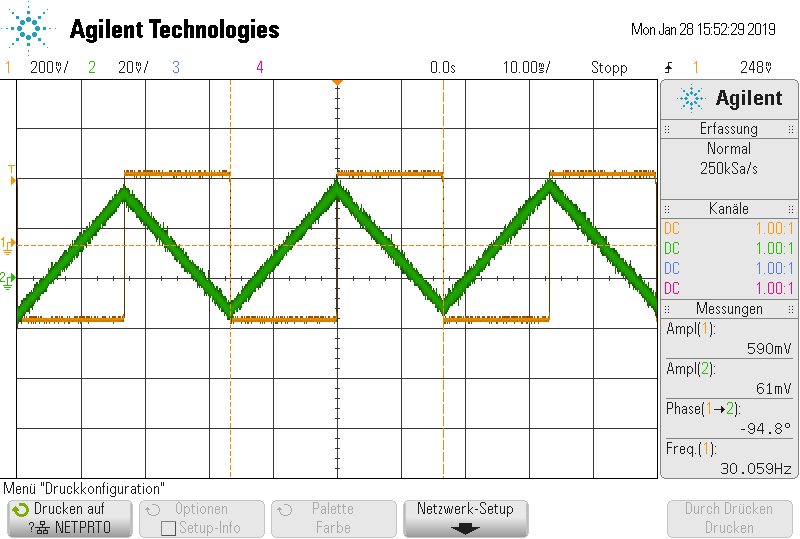
\includegraphics[width=0.8\textwidth]{Schlager/scope_16.png}
  \caption{Das Oszilloskopbild des Umkehr-Integrators bei angelegter Rechteckspannung.}
  \label{fig:int_recht}
\end{figure}
\begin{figure}
  \centering
  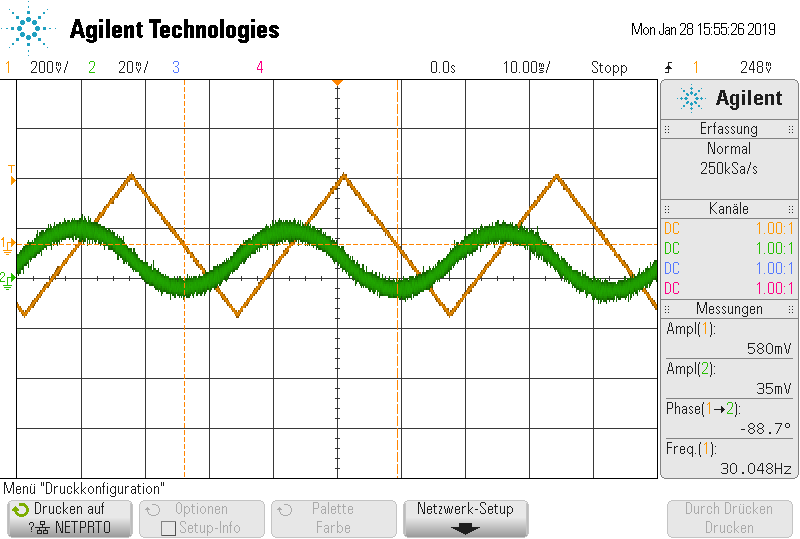
\includegraphics[width=0.8\textwidth]{Schlager/scope_17.png}
  \caption{Das Oszilloskopbild des Umkehr-Integrators bei angelegter Dreiecksspannung.}
  \label{fig:int_drei}
\end{figure}
\begin{figure}
  \centering
  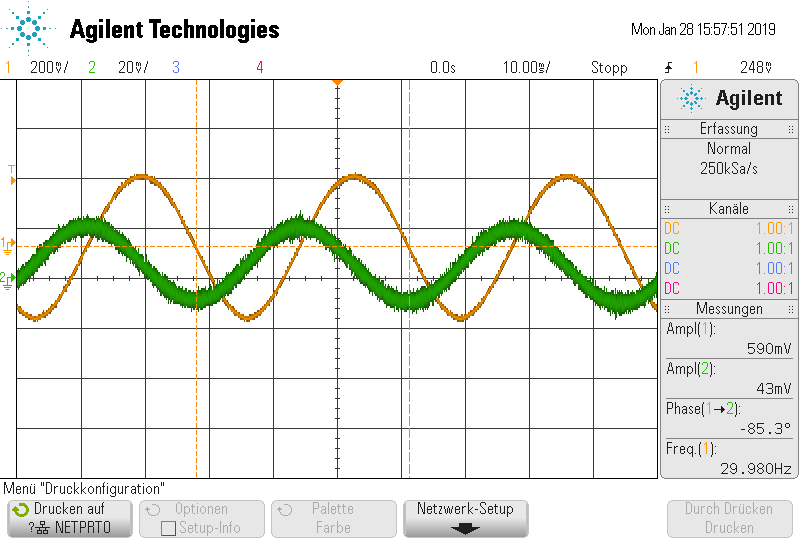
\includegraphics[width=0.8\textwidth]{Schlager/scope_18.png}
  \caption{Das Oszilloskopbild des Umkehr-Integrators bei angelegter Sinusspannung.}
  \label{fig:int_sin}
\end{figure}

Außerdem wird die Verstärkung $V' = U_\text{A}/U_0$ gegen die Kreisfrequenz $\omega$ aufgetragen. Dabei ist die Eingangsspannung sinusförmig. Die Messwerte sind in Tabelle \ref{tab:int_werte} zu finden.
Die Fitfunktion nach Formel \eqref{eqn:???} lautet:
\begin{align}
  V' = \frac{1}{k \omega}.
\end{align}
Aus dem Fit, der zusammen mit den Messwerten in Abbildung \ref{fig:int_fit} zu sehen ist, folgt:
\begin{align*}
  k = \SI{0.062(3)}{\ohm\farad}.
\intertext{Die prozentuale Abweichung von dem nach Formel \eqref{eqn:???} erwarteten Wert beträgt:}
  \Delta_{k, RC} = \SI{36(3)}{\percent}.
\end{align*}

\begin{figure}
  \centering
  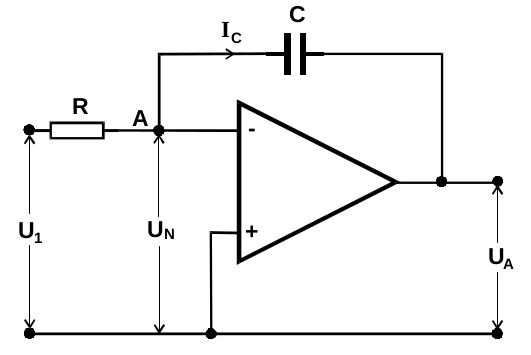
\includegraphics[width=0.8\textwidth]{build/integrator.pdf}
  \caption{Die frequenzabhängige Verstärkung des Umkehr-Integrators bei angelegter Sinusspannung.}
  \label{fig:int_fit}
\end{figure}

\subsection{Umkehr-Differentiator}


% \begin{figure}
%   \centering
%   \includegraphics{build/plotElement.pdf}
%   \caption{Plot.}
%   \label{fig:plot}
% \end{figure}
%
% Tabelle für copy and paste:
% \begin{table}[h]
%   \centering
%   \begin{tabular}{S S}
%     \toprule
%     {$k$} & {$U\:/\:\si{\milli\volt}$}\\
%     \midrule
%     1 & 637.2\\
%     3 & 212.4\\
%     5 & 127.4\\
%     7 & 91.03\\
%     9 & 70.8\\
%     \bottomrule
%   \end{tabular}
%   \caption{Amplituden Rechteckspannung.}
%   \label{tab:rechtampl}
% \end{table}
